\chapter{Tidsplan}
Fra starten af lagde vi en plan over hvornår vi ville udføre de delmål vi havde. Denne plan fremgår af figur \ref{fig:tidsplan1}. Som det kan ses var planen at starte med basic-delmålene og derfra bevæge os ud mod de mere avancerede som liv, hastighed, score, internt koordinatsystem, sværhedsgrader osv. Efterfølgende ville vi implementere et DEXXA Steering Wheel som controller til sjovere styring af spillet.\\
Efter dette ville vi begynde på hvad man kan kalde en finpudsning af spillet, dvs. ordentlig start menu og beskeder hvis spillet vindes eller tabes. \\

Efterfølgende ville vi lave achievements, altså power-up's og power-down's til spillet. Vi fandt lynhurtigt masse potentielle af disse, såsom at strikeren skulle kunne blive bredere/smallere, bolden skulle kunne klistre til strikeren, bolden skulle kunne skydes direkte igennem brikkerne uden at blive reflekteret og størrelsen og hastigheden af bolden skulle kunne ændres osv. Vi havde rent faktisk så mange idéer, at kun tiden satte grænser for hvor mange achievements vi ville implementere. Vi valgte at sætte dette som det tredje sidste punkt i planen, da achievements skulle være en bonus til en allerede spilbart og udfordrende gameplay.\\ \\


\begin{figure}[h!]
\centering
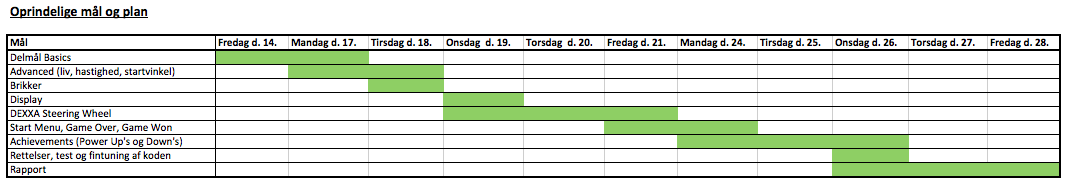
\includegraphics[scale=0.4]{figs/Tidsplan1.png}
\caption{Tidsplan over de forskellige delmål og hvornår de skulle være færdige}
\label{fig:tidsplan1}
\end{figure}